\chapter{Methodology} \label{chap:Methodology}

\begin{figure}[htbp]
  \begin{center}
  \makebox[\textwidth]{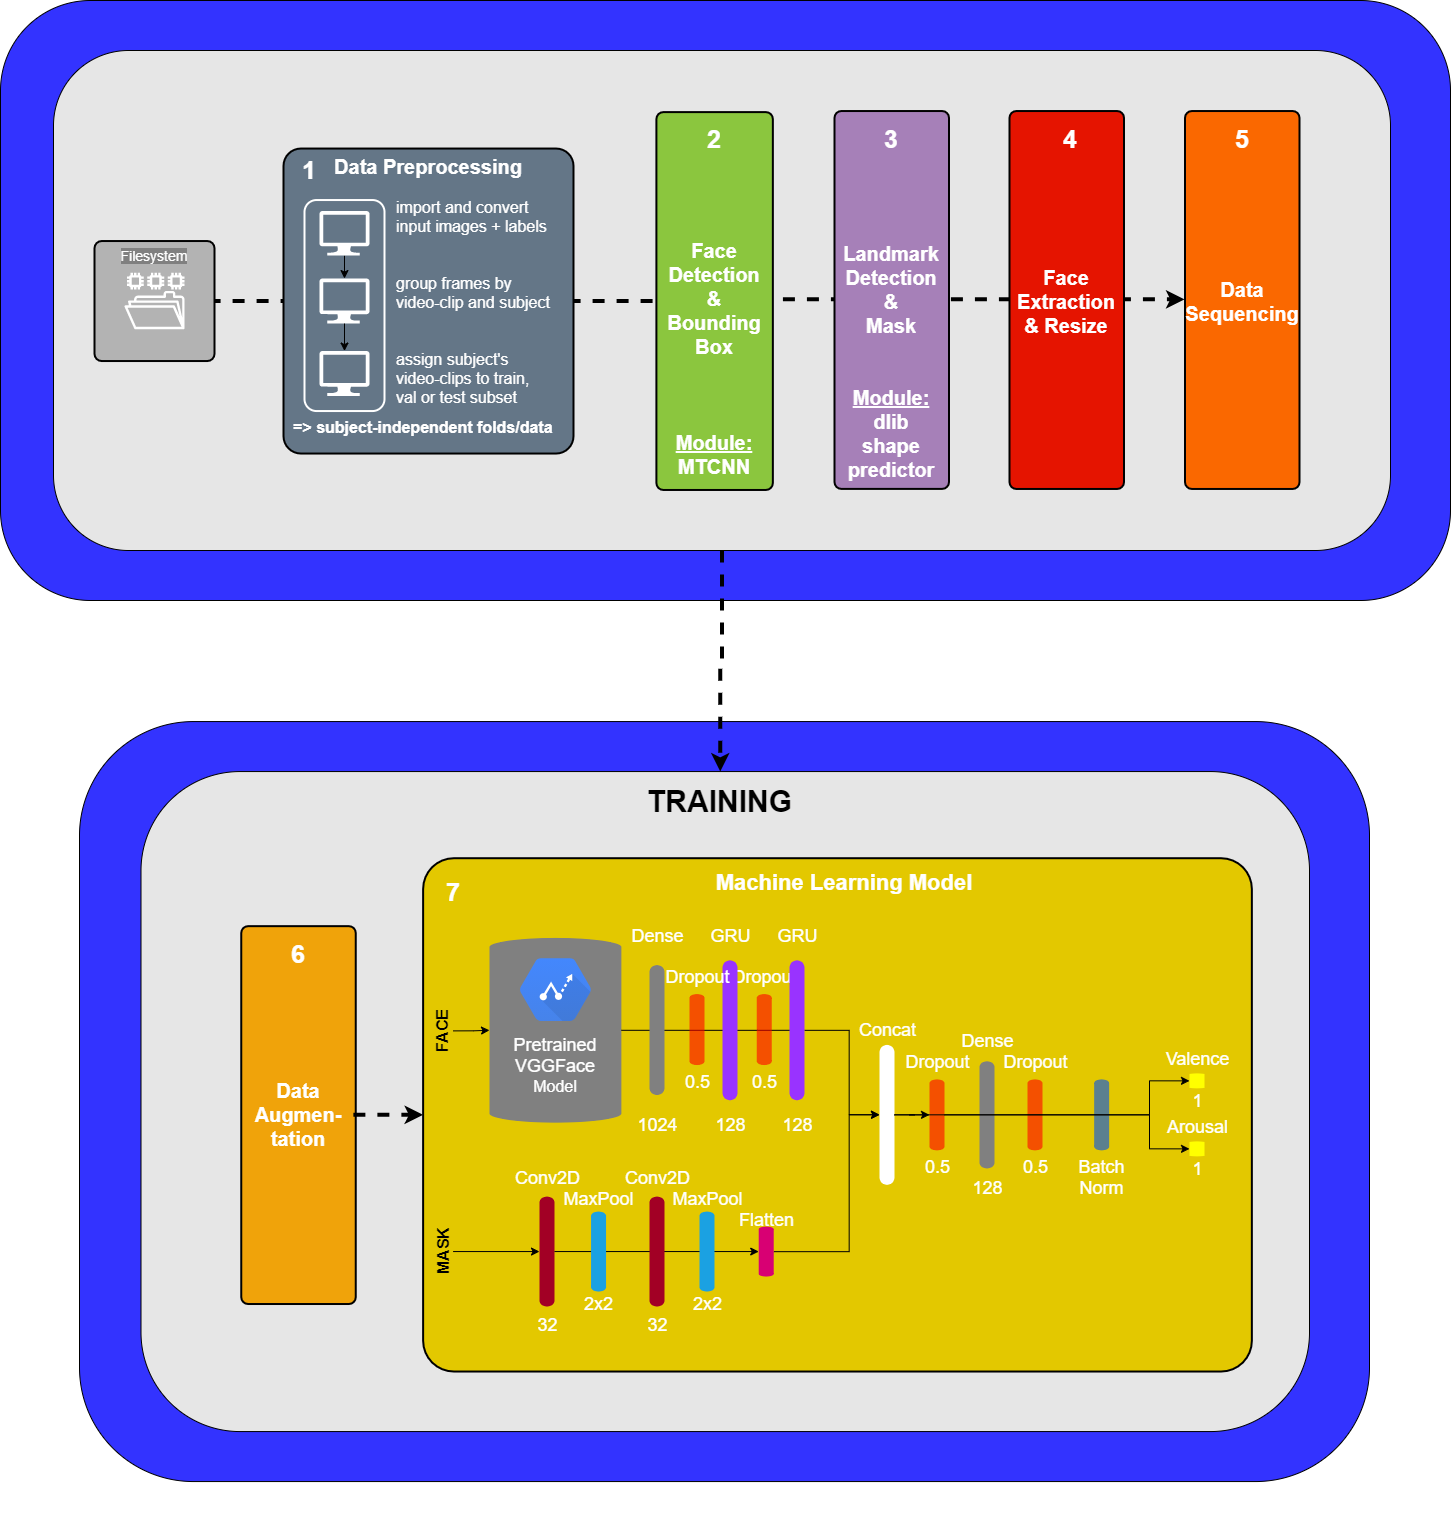
\includegraphics[width=0.85\textwidth]{Figures/EmotionRecognitionInTheWild-RNN_Pipeline.png}}
  \caption[Emotion recognition (ER) pipeline]{This figure shows the emotion recognition pipeline required in this Master's thesis. It consists of six essential steps, starting from reading in data from the file system to the prediction of the emotion through a machine learning model.}
  \label{fig:MachineLearningModelMethods}
  \end{center}
\end{figure}

\noindent This chapter covers the proposed emotion recognition approach in detail. Figure \ref{fig:MachineLearningModelMethods} illustrates the emotion recognition pipeline in this Master's thesis. While step \#1 to step \#5 were performed initially on the whole dataset, step \#6 was applied on a per batch basis during the optimization of the neural network. First, the components of the pipeline are highlighted briefly, afterwards, each component is described in detail along with justification for the design choices in the following sections. 

\begin{enumerate}
    \item Video frames and their labels were imported, grouped by subject and assigned to either the training, validation or test subset. This ensured the creation of subject-independent folds/data.
    \item For each frame the face was detected and a bounding box was determined using a pre-trained network optimized for face detection, namely MTCNN \citep{Zhang:2016:MTCCN}.
    \item Landmarks were detected based on the previously determined bounding box. These landmarks were then saved as a mask in a 2-dimensional image for the usage as an input for the machine learning model.
    \item The face was extracted from the image by cropping it along the borders of the bounding box. The resulting extract was then resized to a 224x224 format.
    \item The extracted faces were put into a sequence of 45 frames for each video-clip.
    \item Data was passed into the machine learning model, consisting of a the pre-trained VGGFace \citep{Cao:2018:VGGFace2} neural network that was extended with a Recurrent Neural Network (RNN) as a custom classifier. In this way, the output features of the VGGFace network for each frame in a video-clip are combined and fed into the RNN which then learns  tempo-spatial aspects of a video-clip. The VGGFace network will be discussed in more details in section \ref{sec:Training&Regularization}.
\end{enumerate}

% Sixth, data augmentation was applied in order to significantly increase the diversity of the images in the underlying dataset.  

%%%%%%%%%%%%%%%%%%%%%%%
\section{Data Preprocessing}
The very first step in the proposed pipeline, as shown in Figure \ref{fig:MachineLearningModelMethods}, is data preprocessing. Here, the input images/frames were imported and converted into the right format. Their corresponding labels, originally in the scale of -10 to +10, were re-scaled to a scale of -1 to +1 in order to fit the chosen 'tanh' activation function of the machine learning model.
\newline\newline
Samples of the input images and their corresponding output labels are shown in Figure \ref{fig:MethodologyPreprocess}. Output labels consist of valence (=expression of how positive or negative an emotion is) and arousal (=expression of how strong or weak an emotion is).
\newline\newline
Furthermore, for the later performed video sampling, frames were already grouped by video-clips and by subject. With this, a subject's video-clips could be assigned to either the training, validation or test subset in a subject-independent manner. 

\begin{figure}[htbp]
  \centering
  \subfloat[V: 0.0, A: +0.5]{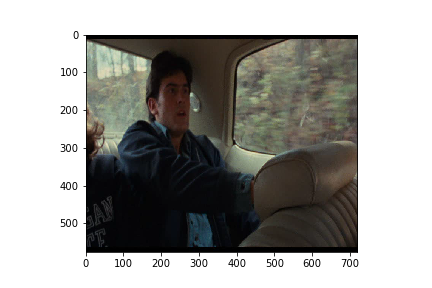
\includegraphics[width=0.5\textwidth]{Figures/001/001_1_00000.png}}
  \hfill
  \subfloat[V: 0.0, A: +0.5]{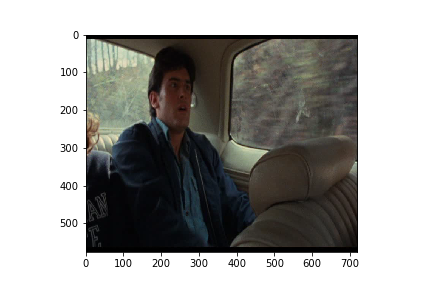
\includegraphics[width=0.5\textwidth]{Figures/001/001_1_00011.png}}
  \hfill
  \subfloat[V: +0.2, A: +0.3]{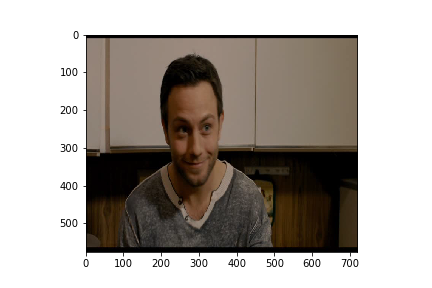
\includegraphics[width=0.5\textwidth]{Figures/002/002_1_00000.png}}
  \hfill
  \subfloat[V: +0.2, A: +0.4]{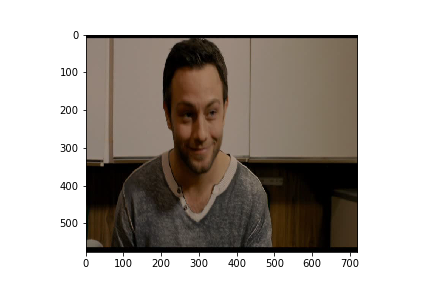
\includegraphics[width=0.5\textwidth]{Figures/002/002_1_00011.png}}
  \hfill
  \subfloat[V: -0.5, A: +0.3]{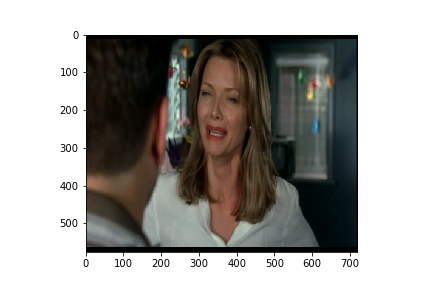
\includegraphics[width=0.5\textwidth]{Figures/576/576_1_00000.png}}
  \hfill
  \subfloat[V: -0.6, A: +0.3]{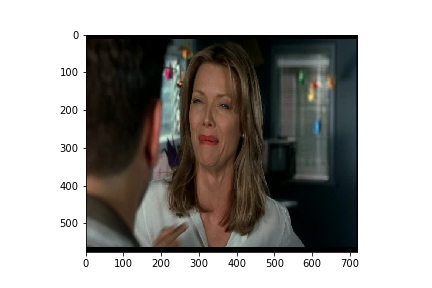
\includegraphics[width=0.5\textwidth]{Figures/576/576_1_00011.png}}
  \caption[ER pipeline step \#1: Preprocessing]{This figure illustrates frames after step \#1 Preprocessing: Frames were preprocessed and samples are displayed together with their corresponding labels, expressed by valence (V) and arousal (A) as values ranging from -1 (V: very negative; A: very calming) to +1 (V: very positive; A: very exciting)}
  \label{fig:MethodologyPreprocess}
\end{figure}


%%%%%%%%%%%%%%%%%%%%%%%%%%%%%%%%%%%%%%%%%%%%%%%%%%
\section{Face Detection} \label{sec:FaceDetection}

\begin{figure}[htbp]
  \centering
  \subfloat[V: 0.0, A: +0.5]{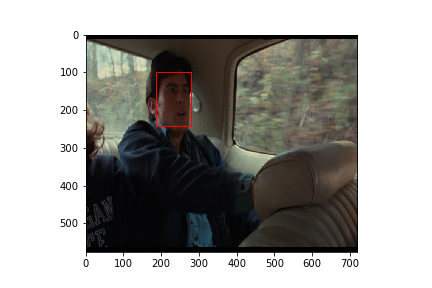
\includegraphics[width=0.5\textwidth]{Figures/001/001_2_00000.png}}
  \hfill
  \subfloat[V: 0.0, A: +0.5]{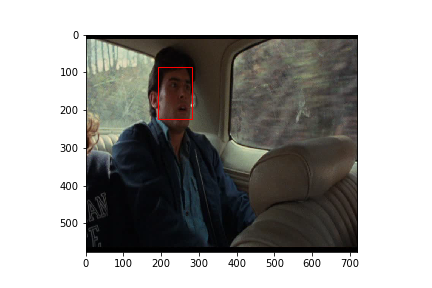
\includegraphics[width=0.5\textwidth]{Figures/001/001_2_00011.png}}
  \hfill
  \subfloat[V: +0.2, A: +0.3]{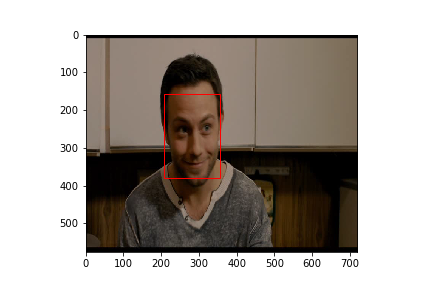
\includegraphics[width=0.5\textwidth]{Figures/002/002_2_00000.png}}
  \hfill
  \subfloat[V: +0.2, A: +0.4]{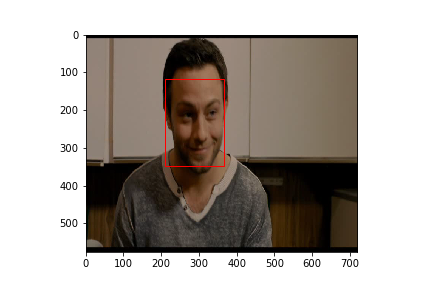
\includegraphics[width=0.5\textwidth]{Figures/002/002_2_00011.png}}
  \hfill
  \subfloat[V: -0.5, A: +0.3]{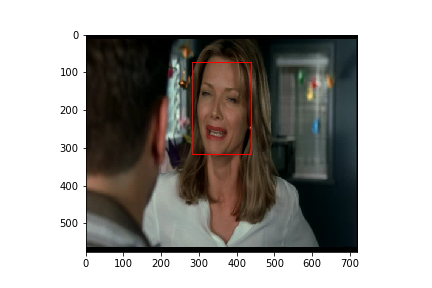
\includegraphics[width=0.5\textwidth]{Figures/576/576_2_00000.png}}
  \hfill
  \subfloat[V: -0.6, A: +0.3]{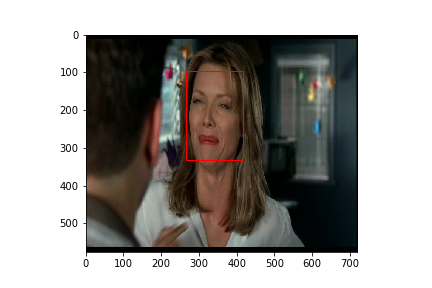
\includegraphics[width=0.5\textwidth]{Figures/576/576_2_00011.png}}
  \caption[ER pipeline step \#2: Face detection \& bounding box]{These images show samples from step \#2 Face detection \& bounding box: The bounding box detected by the MTCNN \citep{Zhang:2016:MTCCN} face detection module is visualized together with their corresponding labels, expressed by valence (V) and arousal (A) as values ranging from -1 (V: very negative; A: very calming) to +1 (V: very positive; A: very exciting)}
  \label{fig:MethodologyBoundingBox}
\end{figure}

The second step in the proposed pipeline involves detecting the faces in each frame of the video. For this, the Multi-Task Cascaded Convolutional Neural Network (MTCNN) by \citet{Zhang:2016:MTCCN} was used. The benefit of this step is three-fold: 1) by cropping the image to fit a person's face the neural network learns only from this input, 2) the bounding box can later on be used as an input to the landmark detection model and 3) the successful detection serves as a criteria for removing frames during the video sampling process.
\newline\newline
The MTCNN \citep{Zhang:2016:MTCCN} model is a pre-trained neural network optimized for the tasks of simultaneous face detection, face alignment, bounding boxing and landmark detection. This makes it ideal for the purpose of determining the face's bounding box in the face of the video frames. In Figure \ref{fig:MethodologyBoundingBox} successful examples of the application of the MTCNN algorithm are shown by overlaying the bounding box on the image.

\vspace{0.5cm}
%%%%%%%%%%%%%%%%%%%%%%%%%%%%
\section{Landmark Detection}
The third step in the proposed pipeline involves the detection of facial landmarks in each frame. This is a preliminary step for the generation of a two-dimensional mask, as it is based on the coordinates of the landmark points.
\newline\newline
This was done using a 'Face Landmark Detection' algorithm based on the work done by \citet{Kazemi:2014:ShapePredictor}. The algorithm is based on an ensemble of regression trees which successively aligns the constructed shape model to the specific features of the the face at hand.
\newline\newline
The input required for the algorithm consists of the frame, as well as coordinates of the face's bounding box. The algorithm's output is made up of 68 facial landmarks of a person's face. Examples of this successful operation are shown in Figure \ref{fig:MethodologyLandmarks} by overlaying the landmark dots on the input image.
\newline\newline
These landmarks were then used to generate a two-dimensional mask. This mask can then be fed as a separate input, next to the image, into the neural network. Such a mask would then enable the network to learn to differentiate the importance of areas in an input image. Results of the generated landmark mask can be seen in Figure \ref{fig:MethodologyMask}.

\begin{figure}[htbp]
  \centering
  \subfloat[V: 0.0, A: +0.5]{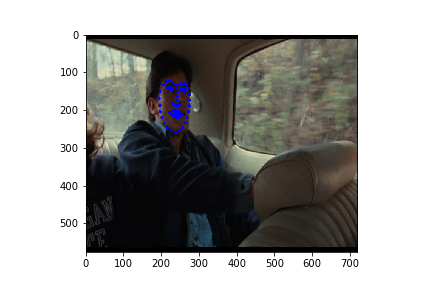
\includegraphics[width=0.5\textwidth]{Figures/001/001_3_00000.png}}
  \hfill
  \subfloat[V: 0.0, A: +0.5]{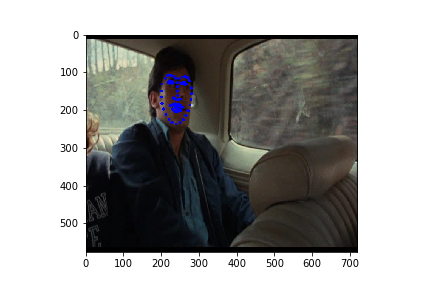
\includegraphics[width=0.5\textwidth]{Figures/001/001_3_00011.png}}
  \hfill
  \subfloat[V: +0.2, A: +0.3]{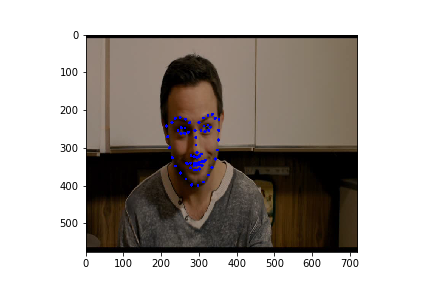
\includegraphics[width=0.5\textwidth]{Figures/002/002_3_00000.png}}
  \hfill
  \subfloat[V: +0.2, A: +0.4]{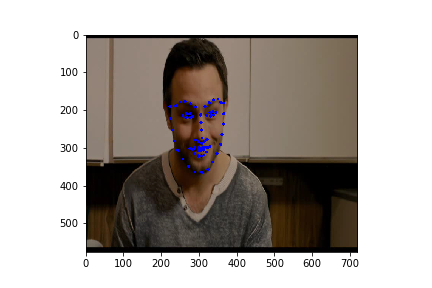
\includegraphics[width=0.5\textwidth]{Figures/002/002_3_00011.png}}
  \hfill
  \subfloat[V: -0.5, A: +0.3]{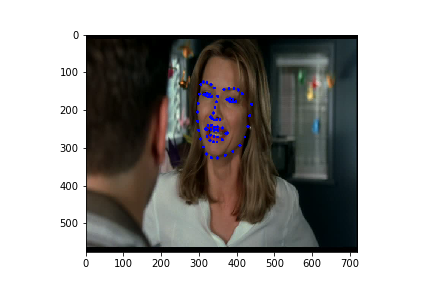
\includegraphics[width=0.5\textwidth]{Figures/576/576_3_00000.png}}
  \hfill
  \subfloat[V: -0.6, A: +0.3]{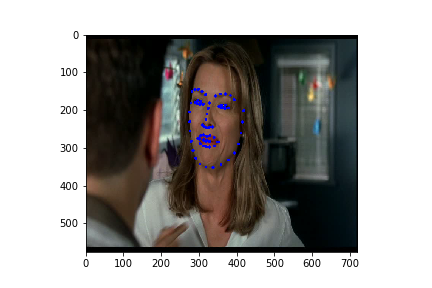
\includegraphics[width=0.5\textwidth]{Figures/576/576_3_00011.png}}
  \caption[ER pipeline step \#3: Landmark detection]{These pictures show sample outputs of step \#3 Landmark detection: Visualization of the landmarks detected by the pre-trained 'Face Landmark Detection' algorithm \citep{Kazemi:2014:ShapePredictor} and their corresponding labels, expressed by valence (V) and arousal (A) as values ranging from -1 (V: very negative; A: very calming) to +1 (V: very positive; A: very exciting)}
  \label{fig:MethodologyLandmarks}
\end{figure}

\begin{figure}[htbp]
  \centering
  \subfloat[V: 0.0, A: +0.5]{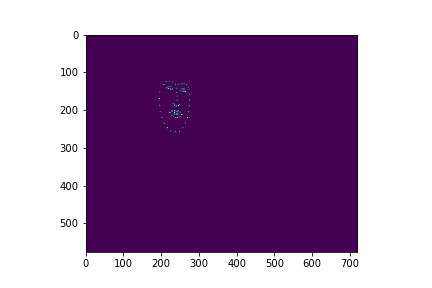
\includegraphics[width=0.5\textwidth]{Figures/001/001_4_00000.png}}
  \hfill
  \subfloat[V: 0.0, A: +0.5]{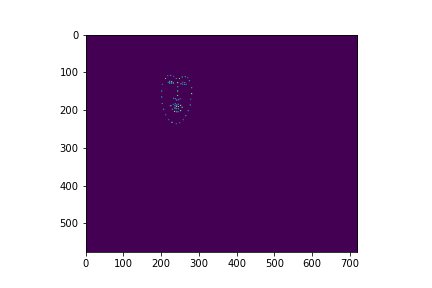
\includegraphics[width=0.5\textwidth]{Figures/001/001_4_00011.png}}
  \hfill
  \subfloat[V: +0.2, A: +0.3]{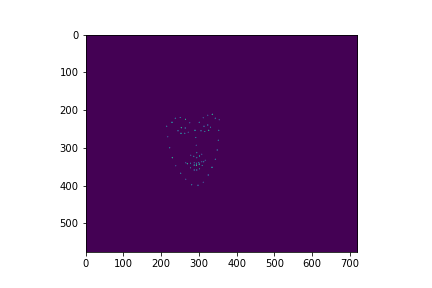
\includegraphics[width=0.5\textwidth]{Figures/002/002_4_00000.png}}
  \hfill
  \subfloat[V: +0.2, A: +0.4]{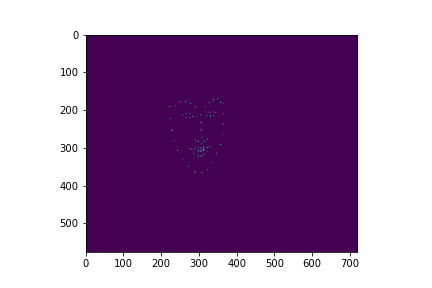
\includegraphics[width=0.5\textwidth]{Figures/002/002_4_00011.png}}
  \hfill
  \subfloat[V: -0.5, A: +0.3]{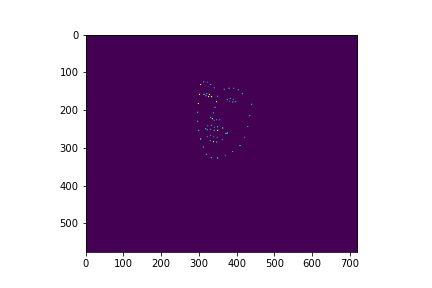
\includegraphics[width=0.5\textwidth]{Figures/576/576_4_00000.png}}
  \hfill
  \subfloat[V: -0.6, A: +0.3]{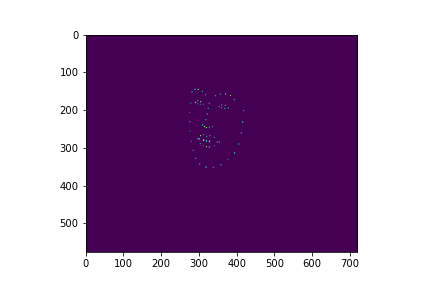
\includegraphics[width=0.5\textwidth]{Figures/576/576_4_00011.png}}
  \caption[ER pipeline step \#3: Mask]{These figures illustrate the outcome of step \#3 Landmark detection: Visualization of the generated mask based on detected landmark points and their corresponding labels, expressed by valence (V) and arousal (A) as values ranging from -1 (V: very negative; A: very calming) to +1 (V: very positive; A: very exciting)}
  \label{fig:MethodologyMask}
\end{figure}


%%%%%%%%%%%%%%%%%%%%%%%%%%%%%%%%%%%%%%%%%%%%%%%%%%%%%
\section{Face Extraction}

\begin{figure}[htbp]
  \centering
  \subfloat[V: 0.0, A: +0.5]{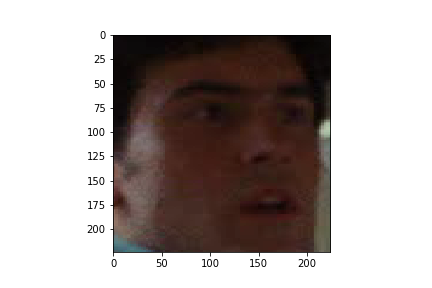
\includegraphics[width=0.5\textwidth]{Figures/001/001_5_00000.png}}
  \hfill
  \subfloat[V: 0.0, A: +0.5]{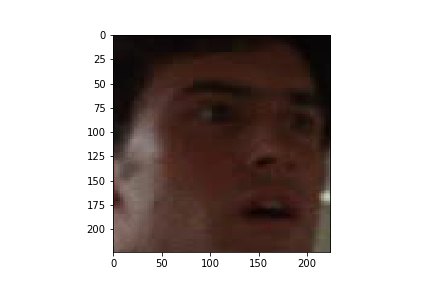
\includegraphics[width=0.5\textwidth]{Figures/001/001_5_00011.png}}
  \hfill
  \subfloat[V: +0.2, A: +0.3]{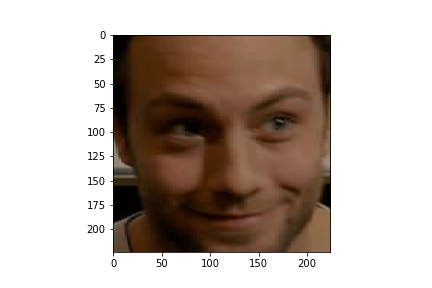
\includegraphics[width=0.5\textwidth]{Figures/002/002_5_00000.png}}
  \hfill
  \subfloat[V: +0.2, A: +0.4]{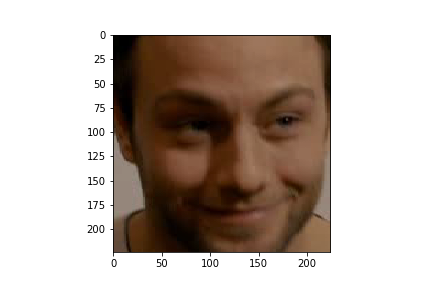
\includegraphics[width=0.5\textwidth]{Figures/002/002_5_00011.png}}
  \hfill
  \subfloat[V: -0.5, A: +0.3]{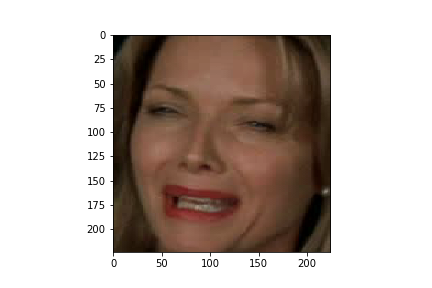
\includegraphics[width=0.5\textwidth]{Figures/576/576_5_00000.png}}
  \hfill
  \subfloat[V: -0.6, A: +0.3]{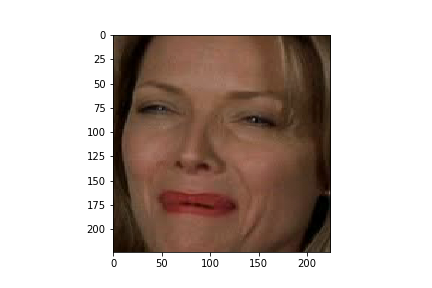
\includegraphics[width=0.5\textwidth]{Figures/576/576_5_00011.png}}
  \caption[ER pipeline step \#4: Face extraction]{The images show the faces as part of step \#4 Face extraction: Visualization of the extracted face and their corresponding labels, expressed by valence (V) and arousal (A) as values ranging from -1 (V: very negative; A: very calming) to +1 (V: very positive; A: very exciting)}
  \label{fig:MethodologyExtraction}
\end{figure}

\begin{figure}[htbp]
  \centering
  \subfloat[V: 0.0, A: +0.5]{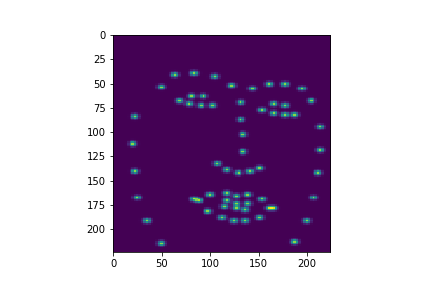
\includegraphics[width=0.5\textwidth]{Figures/001/001_5_2_00000.png}}
  \hfill
  \subfloat[V: 0.0, A: +0.5]{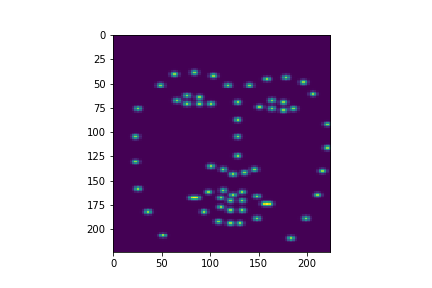
\includegraphics[width=0.5\textwidth]{Figures/001/001_5_2_00011.png}}
  \hfill
  \subfloat[V: +0.2, A: +0.3]{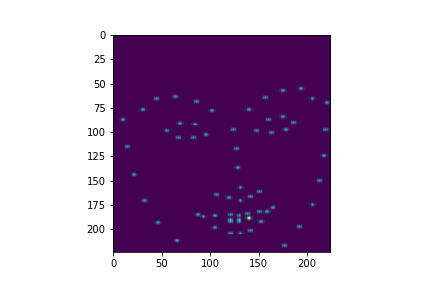
\includegraphics[width=0.5\textwidth]{Figures/002/002_5_2_00000.png}}
  \hfill
  \subfloat[V: +0.2, A: +0.4]{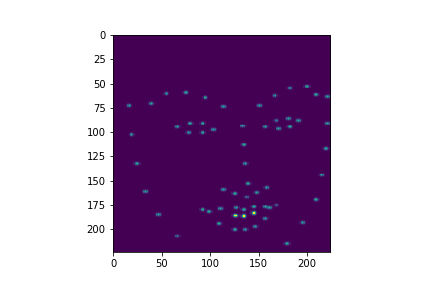
\includegraphics[width=0.5\textwidth]{Figures/002/002_5_2_00011.png}}
  \hfill
  \subfloat[V: -0.5, A: +0.3]{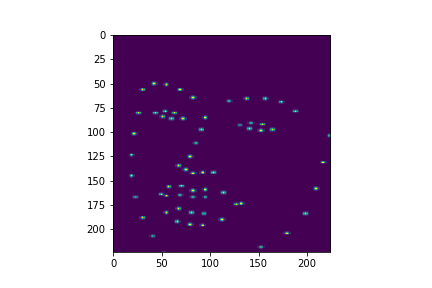
\includegraphics[width=0.5\textwidth]{Figures/576/576_5_2_00000.png}}
  \hfill
  \subfloat[V: -0.6, A: +0.3]{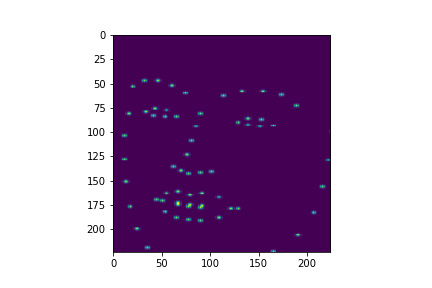
\includegraphics[width=0.5\textwidth]{Figures/576/576_5_2_00011.png}}
  \caption[ER pipeline step \#4: Mask extraction]{The figures display the masks as port of step \#4 Mask extraction: Visualization of the extracted mask and their corresponding labels, expressed by valence (V) and arousal (A) as values ranging from -1 (V: very negative; A: very calming) to +1 (V: very positive; A: very exciting)}
  \label{fig:MethodologyExtractionMask}
\end{figure}

\noindent In this step, faces are extracted from the original input image based on the face's bounding box. The same extraction is performed for the mask containing the landmarks. This is valuable as it removes unimportant information/features of the image's background which could otherwise negatively affect the learning process.
\newline\newline
This step was conducted by simply cropping the face along the border lines of the face's bounding box. The output is again a image with a dimension of 224x224 pixels that displays the inner area of the bounding box, namely the person's face. Example outputs are illustrated in Figure \ref{fig:MethodologyExtraction}. At the same time, also the mask had to be cropped along the same border lines of the face's bounding box. Results of this are presented in Figure \ref{fig:MethodologyExtractionMask}.



%%%%%%%%%%%%%
\section{Video Sampling}
Video-clips for each data subset (train, validation and test) were sampled by duplicating or removing frames so that each video-clip contained exactly 45 frames with successfully extracted faces. This step is important, as it allows the input to be fed into a Recurrent Neural Network (RNN) which is then able to extract information from tempo-spatial changes.
\newline\newline
The number of 45 frames per video-clip was chosen slightly below the median number of frames per video-clip (= 45.5). Video Sampling was done by duplicating or removing frames at a regular interval depending on the ratio between the actual number of frames per video-clip and the desired sequence length of 45. The same actions were also applied to the corresponding face masks.
\newline\newline
Overall, the video sampling step resulted in an reduction of the dataset size from around 30.050 frames (average number of 50.1 frames; median number of 45.5 frames) to 27.000 frames (average \& median number of 45 frames per video-clip). Additionally to that, another 27.000 images are the result of the same actions applied to the corresponding masks.


%%%%%%%%%%%%%%%%%%%%%%%%%%%%%%%%%%%%%%%%%%%%%%%%%%%%%
\section{Machine Learning Model for Emotion Recognition}
In the final step of the proposed pipeline, the augmented frames are fed into the machine learning model for training on the emotion recognition challenge. The model's architecture, consisting of the pre-trained VGGFace model \citep{Cao:2018:VGGFace2} and a custom classifier, can be seen in Figure \ref{fig:MachineLearningModel}.
\newline\newline
The VGGFace model architecture, is based on the famous ResNet-50 convolutional neural network which the authors \citet{Cao:2018:VGGFace2} pre-trained on a large-scale face dataset, named VGGFace2. The dataset contains about 3.31 million images of 9131 subjects and poses, which provided a wide variety of poses, ages, etc. When the VGGFace2 paper, written by \citet{Cao:2018:VGGFace2}, was published in \citeyear{Cao:2018:VGGFace2}, it exceeded the performance of previous state-of-the-art by a large margin \citep{Cao:2018:VGGFace2}.\newline

\begin{figure}[htbp]
  \begin{center}
  \makebox[\textwidth][c]{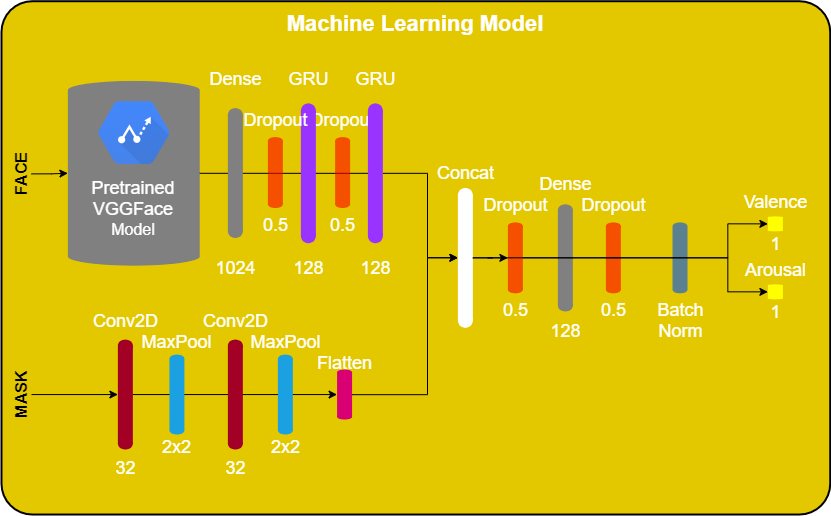
\includegraphics[width=0.8\textwidth]{Figures/MachineLearningModel.png}}
  \caption[ER pipeline step \#6: Machine learning model]{The figure shows a machine learning model consisting of a pre-trained VGGFace network and a custom added RNN. The face's mask is processed through a parallel Convolutional Neural Network. Both outputs are connected and contribute toward the recognition of valence and arousal.}
  \label{fig:MachineLearningModel}
  \end{center}
\end{figure}

\noindent The utilization of a pre-trained neural network is often referred to as transfer learning. Instead of training the model from scratch, transfer learning allows to start the training process from patterns that have already been learned by solving a different problem \citep{Pan:2010:SurveyOnTransferLearning}.
\newline\newline
In this work, a version of the VGGFace model was used that had been pre-trained on the VGGFace2 dataset \citep{Cao:2018:VGGFace2} for the task of face identification. The pre-trained model was then further fine-tuned on the AFEW-VA dataset \citep{Kossaifi:2017:AFEW-VADatabase}. In this way, learnt patterns about facial features from the face identification task were used to kick-start the learning for emotion recognition from there. 
\newline\newline
A noteworthy architectural change was the removal of the last fully-connected layers at the end of VGGFace. For this work, these layers were replaced with another classifier in order to learn the correlation between facial features and their target labels for the emotion recognition task. The architecture of the newly added classifier, as shown in Figure \ref{fig:MachineLearningModel}, includes a Recurrent Neural Network (RNN) for capturing tempo-spatial information.
\newline\newline
In summary, this chapter presented the methods of the proposed approach that are required to predict the emotional values of valence and arousal from a raw input image. Before training a machine learning model on the emotion recognition challenge at hand, an image had to pass through the following steps: Data preprocessing, face detection, landmark detection, face extraction, and video sampling. A highlight of this approach is the utilization of landmarks in the form of a two dimensional mask which was then fed into the machine learning model as a separate input.



